\documentclass{beamer}
\usecolortheme{dove}
\setbeamertemplate{navigation symbols}{}
\usepackage{amsmath,amssymb,amsfonts,amsthm, multicol, subfigure, color}
\usepackage{bm}
\usepackage{graphicx}
\usepackage{tabularx}
\usepackage{booktabs}
\usepackage{hyperref}
\usepackage{pdfpages}
\usepackage{xcolor}
\definecolor{seagreen}{RGB}{46, 139, 87}
\def\independenT#1#2{\mathrel{\rlap{$#1#2$}\mkern2mu{#1#2}}}
\newcommand\indep{\protect\mathpalette{\protect\independenT}{\perp}}
\def\log{\text{log}}
\newcommand\logit{\text{logit}}
\newcommand\iid{\stackrel{\text{iid}}{\sim}}
\newcommand\E{\text{E}}
\newcommand\V{\text{V}}
\renewcommand\P{\text{P}}
\newcommand{\Cov}{\text{Cov}}
\newcommand{\Cor}{\text{Cor}}
\newcommand\doop{\text{do}}


\usepackage{stackrel}
\usepackage{tikz}
\usetikzlibrary{arrows,shapes.arrows,positioning,shapes,patterns,calc}
\newcommand\slideref[1]{\vskip .1cm \tiny \textcolor{gray}{{#1}}}
\newcommand\red[1]{\color{red}#1}
\newcommand\blue[1]{\color{blue}#1}
\newcommand\gray[1]{\color{gray}#1}
\newcommand\seagreen[1]{\color{seagreen}#1}
\newcommand\purple[1]{\color{purple}#1}
\newcommand\orange[1]{\color{orange}#1}
\newcommand\black[1]{\color{black}#1}
\newcommand\white[1]{\color{white}#1}
\newcommand\teal[1]{\color{teal}#1}
\newcommand\magenta[1]{\color{magenta}#1}
\newcommand\Fuchsia[1]{\color{Fuchsia}#1}
\newcommand\BlueGreen[1]{\color{BlueGreen}#1}
\newcommand\bblue[1]{\textcolor{blue}{\textbf{#1}}}
\newcommand\bred[1]{\textcolor{red}{\textbf{#1}}}
\newcommand\bgray[1]{\textcolor{gray}{\textbf{#1}}}
\newcommand\bgreen[1]{\textcolor{seagreen}{\textbf{#1}}}
\newcommand\bref[2]{\href{#1}{\color{blue}{#2}}}
\colorlet{lightgray}{gray!40}
\pgfdeclarelayer{bg}    % declare background layer for tikz
\pgfsetlayers{bg,main} % order layers for tikz
\newcommand\mycite[1]{\begin{scriptsize}\textcolor{darkgray}{(#1)}\end{scriptsize}}
\newcommand{\tcframe}{\frame{
%\small{
\only<1|handout:0>{\tableofcontents}
\only<2|handout:1>{\tableofcontents[currentsection]}}
%}
}

\setbeamertemplate{footline}[frame number]


\usepackage[round]{natbib}
\bibliographystyle{humannat-mod}
\setbeamertemplate{enumerate items}[default]
\usepackage{mathtools}

\newcommand{\goalsframe}{\begin{frame}{Learning goals for today}
At the end of class, you will be able to:
\begin{enumerate}
\item Explain why exchangeability holds in randomized experiments
\item Understand why exchangeability allows for direct estimation of causal effects
\end{enumerate} \vskip .2in
\end{frame}}

\title{Randomized experiments}
\author{INFO/STSCI/ILRST 3900: Causal Inference}
\date{29 Aug 2023}

\begin{document}

\maketitle

\goalsframe

\section{Quick Refresher}

\begin{frame}{Potential outcome notation review}
\begin{itemize}
\item We typically use $i$ to denote a generic unit in our study
\item $Y_i$ is the observed outcome for unit $i$
\item $A_i$ is treatment received by unit $i$
\item We typically use $a$ to denote a generic treatment in our study
\item $Y^a_i$ denotes the outcome we would have observed for unit $i$ if assigned treatment value $a$
\end{itemize}
\end{frame}


\begin{frame}{Potential outcome exercise}
\begin{itemize}
\item We observe that Martha ate a Mediterranean diet, and we observe that Martha survived.
\\ Suppose Martha had eaten a standard diet, we would have observed that Martha survived. 
\item We observe that Ezra ate a standard diet, and we observe that Ezra did not survive
\\ Suppose Ezra had eaten a Mediterranean diet, we would have observed that Ezra survived. 
\end{itemize}
\pause

\vspace{1em}

Assuming \emph{consistency}, what is $A_i$, $Y_i$, $Y_i^{\texttt{MedDiet}}$ and $Y_i^{\texttt{StanDiet}}$
\begin{itemize}
\item When $i = \text{Martha}$?
\item When $i = \text{Ezra}$? 
\end{itemize}


\end{frame}


\begin{frame}{Potential outcome exercise}
Suppose we know the following pieces of information:
{\small
\begin{itemize}
\item We observe that Martha ate a Mediterranean diet, and we observe that Martha survived.
\\ Suppose Martha had eaten a standard diet, we would have observed that Martha survived. 
\item We observe that Ezra ate a standard diet, and we observe that Ezra did not survive
\\ Suppose Ezra had eaten a Mediterranean diet, we would have observed that Ezra survived. 
\end{itemize}
}

\begin{table}
  \renewcommand*{\arraystretch}{2}
\begin{tabular}[t]{c|c|c| c|c}
  & $A_i$ & $Y_i$ & $Y_i^{\text{a = Med}}$ & $Y_i^{\text{a = Stan}}$\\
\hline
Martha & \qquad \qquad \qquad & \qquad \qquad \qquad & \qquad & \qquad\\ \hline
Ezra & \qquad \qquad & \qquad \qquad & \qquad & \qquad\\
\end{tabular}
\end{table}

\end{frame}


\section{Randomized experiments: Two key benefits}



\begin{frame}{Randomized experiments}

\begin{figure}
    \centering
    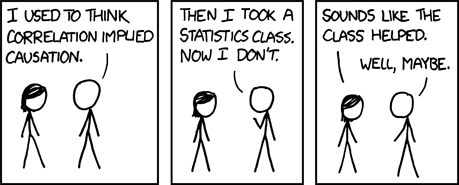
\includegraphics[scale = .7]{figures/correlation.png}\footnote{\url{https://xkcd.com/552/}}
\end{figure}
\end{frame}

\begin{frame}{Randomized experiments}
\begin{figure}
    \centering
    
\includegraphics[scale = .3]{figures/goldStandard.png}
\end{figure}
    
\end{frame}

\begin{frame}{Fundamental problem of causal inference}
\begin{itemize}
     \item Randomized experiments are the gold standard for estimating causal effects
    \item Fundamental problem of causal inference is that we don't observe counterfactual outcomes
    \item Data is still missing in random experiments
\end{itemize}

\begin{table}\footnotesize
    \centering

\begin{tabular}[t]{c|c| c|c|c}
\toprule
  & A & $Y^{a=1}$ & $Y^{a=0}$ & $Y^{a=1} - Y^{a=0}$\\
\midrule
Ind 1 & 0 & ? & 0 & ?\\
Ind 2 & 0 & ? & 1 & ?\\
Ind 3 & 0  & ? & 0 & ?\\
Ind 4 &1 & 1 & ? & ?\\
Ind 5 & 1 & 0 & ? & ?\\
Ind 6 & 1 & 1 & ? & ?\\
\bottomrule
\end{tabular}
\end{table}

\pause 
\begin{itemize}
    \item Why do randomized experiments ``work''?
\end{itemize}
    
\end{frame}



\begin{frame}{What can go wrong?}
Suppose we have data gathered by surveying individuals in Fall of 2021
    \begin{itemize}
        \item Whether the individual was vaccinated for Covid\\
        $A_i = 1$ if vaccinated, $A_i = 0$ if not vaccinated
        \item Whether the individual tested positive for Covid in 2021\\
        $Y_i = 1$ if positive test, $Y_i = 0$ if no positive test
     \end{itemize}



\end{frame}



\begin{frame}{What can go wrong?}

{\large\textbf{Left side of class}} 
     \begin{itemize}
         \item Of the individuals who are \textbf{vaccinated} ($A_i = 1$), 50\% had a positive Covid test ($Y_i = 1$)
         \item Of the individuals who are \textbf{not vaccinated} ($A_i = 0$), 70\% had a positive Covid test ($Y_i = 1$) 
         \item How might a vaccine skeptic explain the data? 
\end{itemize}
\pause
\vspace{1em}
{\large\textbf{Right side of class}} 
     \begin{itemize}
         \item Of the individuals who are \textbf{vaccinated} ($A_i = 1$), 70\% had a positive Covid test ($Y_i = 1$)
         \item Of the individuals who are \textbf{not vaccinated} ($A_i = 0$), 50\% had a positive Covid test ($Y_i = 1$) 
         \item How might a vaccine advocate explain the data? 
\end{itemize}






\end{frame}


\begin{frame}{Randomized experiment}
Experiment designed by Pfizer \textbf{randomly assign} each individual (43,000 total) into two groups\footnote{Polack et. al. NEJM 2020}:
\begin{itemize}
        \item Two doses of BNT162b2 vaccine 21 days apart
        \item Two doses of placebo 21 days apart
        \item Whether a positive Covid test was recorded between 7 days and 14 weeks after the injection
\end{itemize}
\vspace{1em}

\pause
     \begin{itemize}
         \item Of the individuals who were given the vaccine ($A_i = 1$), 0.04\% had a positive Covid test ($Y_i = 1$)
         \item Of the individuals who were given the placebo ($A_i = 0$), 0.9\% had a positive Covid test ($Y_i = 1$)
         \item Individuals who received the placebo were $\approx 20$ times more likely to get Covid 
     \end{itemize}

\pause \vspace{1em}
\textbf{Do the skeptics objections still hold?}


\end{frame}



\begin{frame}{Why experiments ``work''}

\begin{figure}
    \centering
    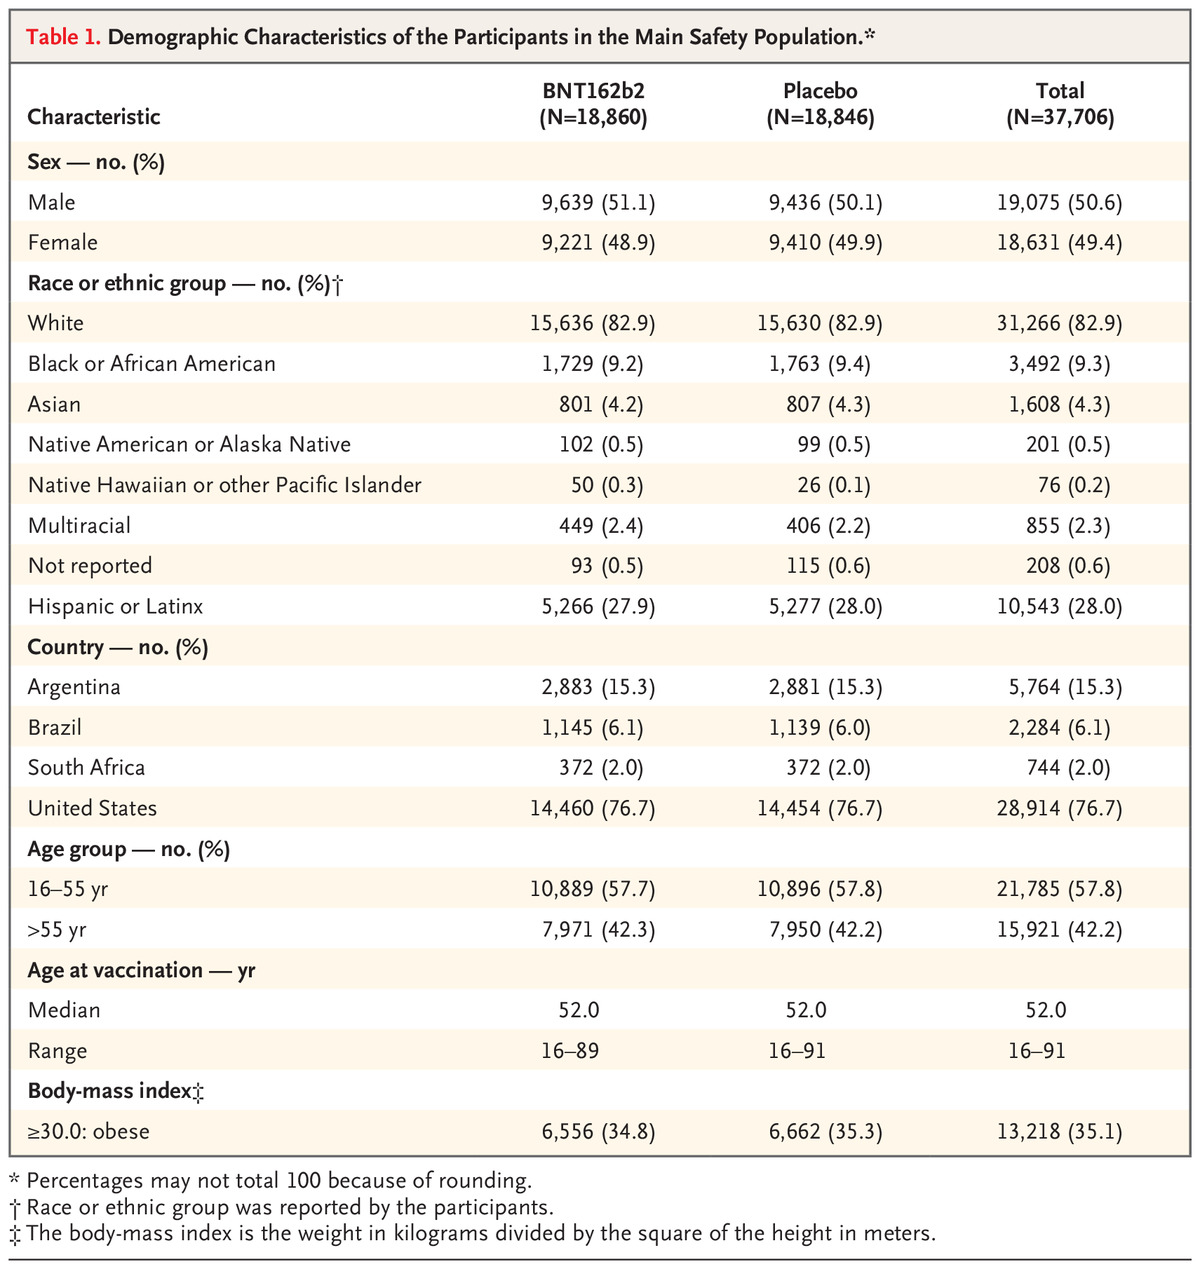
\includegraphics[scale = .18]{figures/pfizer_balance.jpg}
\end{figure}

\end{frame}



\begin{frame}{Why experiments ``work''}

In random experiments, the distribution of \textbf{potential outcomes} for those who are treated and those who are not treated (control group) are similar!

\pause
\vspace{2em}
This is a concept called \textbf{exchangeability}
\pause

\vspace{1em}
Sometimes also referred to as \textbf{exogenous}\hspace{1cm} $\underbrace{exo}_{\text{outside}} \cdot \underbrace{genous}_{\text{to produce}}$


\end{frame}








\begin{frame}{Exchangeability}
\textbf{Definition:} Exchangeability means that the potential outcomes, $Y^{a=1}$ and $Y^{a = 0}$, are independent of the observed treatment ($A$)
\pause
\vspace{1em}

{\small 
\begin{itemize}
    \item Two random variables are \textbf{independent} if the outcome of one does not give any information about the outcome of the other
    \pause 
    \item What we would have observed if an individual was given the treatment ($Y^{a = 1}$) is independent of whether or not the individual actually received treatment 
    \item What we would have observed if an individual was not given the treatment ($Y^{a = 0}$) is independent of whether or not the individual actually received treatment  
    \pause 
     \item Exchangeability means that the \textbf{potential} outcomes $Y^a$ are independent of the observed treatment
    \item Exchangeability does \textbf{not} mean that the \textbf{observed} outcome $Y$ is independent of the observed treatment!
\end{itemize}
}


\end{frame}


\begin{frame}{Exchangeability}
$A = 1$ means vaccinated; $A = 0$ means unvaccinated\\
$Y = 1$ means covid; $Y = 0$ means no covid;

\begin{table}
\begin{tabular}[t]{c|c| c|c|c}
\toprule
& $Y^{a=1}$ & $Y^{a=0}$ & $A$ & $Y$\\
\midrule
Low Risk 1 & 0 & 0 & ? & ?\\
Low Risk 2 & 0 & 0 & ? & ?\\
High Risk 3 & 0 & 1 & ? & ?\\
High Risk 4 & 0 & 1 & ? & ?\\
\bottomrule
\end{tabular}
\end{table}


\pause 
\[\text{Average Causal Effect} =\underbrace{\E(Y^{a = 1})}_{0} - \underbrace{\E(Y^{a = 0})}_{1/2} = -1/2 \]
    

\end{frame}



\begin{frame}{Exchangeability}
$A = 1$ means vaccinated; $A = 0$ means unvaccinated\\
$Y = 1$ means covid; $Y = 0$ means no covid;
\begin{table}
\begin{tabular}[t]{c|c| c|c|c}
\toprule
& $Y^{a=1}$ & $Y^{a=0}$ & $A$ & $Y$\\
\midrule
Low Risk 1 & {\color{lightgray}0} & 0 & 0 & 0\\
Low Risk 2 &{\color{lightgray}0} & 0 & 0 & 0\\
High Risk 3 & 0 & {\color{lightgray}1} & 1 & 0\\
High Risk 4 & 0 & {\color{lightgray}1} & 1 & 0\\
\bottomrule
\end{tabular}
\end{table}

\[\text{Average Causal Effect} =\underbrace{\E(Y^{a = 1})}_{0} - \underbrace{\E(Y^{a = 0})}_{1/2} = -1/2 \]

Suppose Low Risk choose $A_i = 0$ and High Risk choose $A_i = 1$ so the potential outcomes are not independent of the observed treatment
\[\underbrace{\E(Y \mid A = 1)}_{\text{observed unvac}} - \underbrace{\E(Y \mid A = 0)}_{\text{observed unvac}} = 0 \]

\end{frame}


\begin{frame}{Exchangeability}
$A = 1$ means vaccinated; $A = 0$ means unvaccinated\\
$Y = 1$ means covid; $Y = 0$ means no covid;
\begin{table}
\begin{tabular}[t]{c|c| c|c|c}
\toprule
& $Y^{a=1}$ & $Y^{a=0}$ & $A$ & $Y$\\
\midrule
Low Risk 1 & {\color{lightgray}0} & 0 & 1 & 0\\
Low Risk 2 & 0 & {\color{lightgray}0} & 0 & 0\\
High Risk 3 & {\color{lightgray}0} & 1 & 1 & 1\\
High Risk 4 & 0 & {\color{lightgray}1} & 0 & 0\\
\bottomrule
\end{tabular}
\end{table}

\[\text{Average Causal Effect} =\underbrace{\E(Y^{a = 1})}_{0} - \underbrace{\E(Y^{a = 0})}_{1/2} = -1/2 \]
\pause 
\[\underbrace{\E(Y \mid A = 1)}_{\text{observed vac}} - \underbrace{\E(Y \mid A = 0)}_{\text{observed unvac}} = -1/2 \]






\end{frame}




\begin{frame}{Exchangeability}
In mathematical notation, exchangeability means

\vspace{1em}

\[\underbrace{Y^{a = 1}, Y^{a = 0}}_{\text{potential outcomes}} \indep \underbrace{A}_{\text{observed treatment}} \]




\end{frame}

\begin{frame}{Why is exchangeability good?}
The average causal effect (ACE) is the difference in average outcome that would occur if everyone is treated compared to the average outcome that would occur if no-one is treated   

\vspace{1em}

\[
        \text{ACE} = 
        \underbrace{\E(Y^{a = 1})}_{\text{if everyone is treated}} - \underbrace{\E(Y^{a = 0} )}_{\text{if no-one is treated}} \] 
\pause

\vspace{1em}

The problem is, we only know
\begin{itemize}
    \item  $\E(Y^{a=1} \mid A = 1)$, the average $Y^{a=1}$ among individuals who are actually treated
    \item $\E(Y^{a=0} \mid A = 0)$, the average $Y^{a=0}$ among individuals who are actually not treated
\end{itemize}


\end{frame}


\begin{frame}{Why is exchangeability good?}
When exchangeability is true, it implies

\[\underbrace{\E(Y^{a = 1}  \mid A = 1)}_{\text{Within treated}} = \underbrace{\E(Y^{a = 1}  \mid A = 0)}_{\text{Within not treated}} = \underbrace{\E(Y^{a = 1} )}_{\text{everyone}}  \]


\pause

\vspace{2em}
This allows us to identify the average causal effect (ACE)
\[
        \text{ATE} = 
        \underbrace{\E(Y^{a = 1} )}_{\text{if everyone is treated}} - \underbrace{\E(Y^{a = 0} )}_{\text{if no-one is treated}} \] because we can plug-in 
        \[\underbrace{\E(Y^{a = 1} \mid A = 1)}_{\substack{\text{outcomes for people who} \\ \text{are \textbf{actually} treated}}} \quad \text{ 
        and } \quad  \underbrace{\E(Y^{a = 0} \mid A = 0)}_{\substack{\text{outcomes for people who} \\ \text{are \textbf{actually} not treated}}}\]

\end{frame}





\goalsframe

\end{document}

